\section{Data}
We present real world data regarding costs per meter for various data as well as power cables. Moreover, many different LCUs and trench/installation costs are provided for which we can test our heuristics on. The experiments are running on the PS10 solar tpower power plant instance \cite{osuna_2001,osuna_2006} for which the coordinates are provided, a sketch of this instance can be seen in \cref{fig:ps10}.

\begin{figure}[H]
  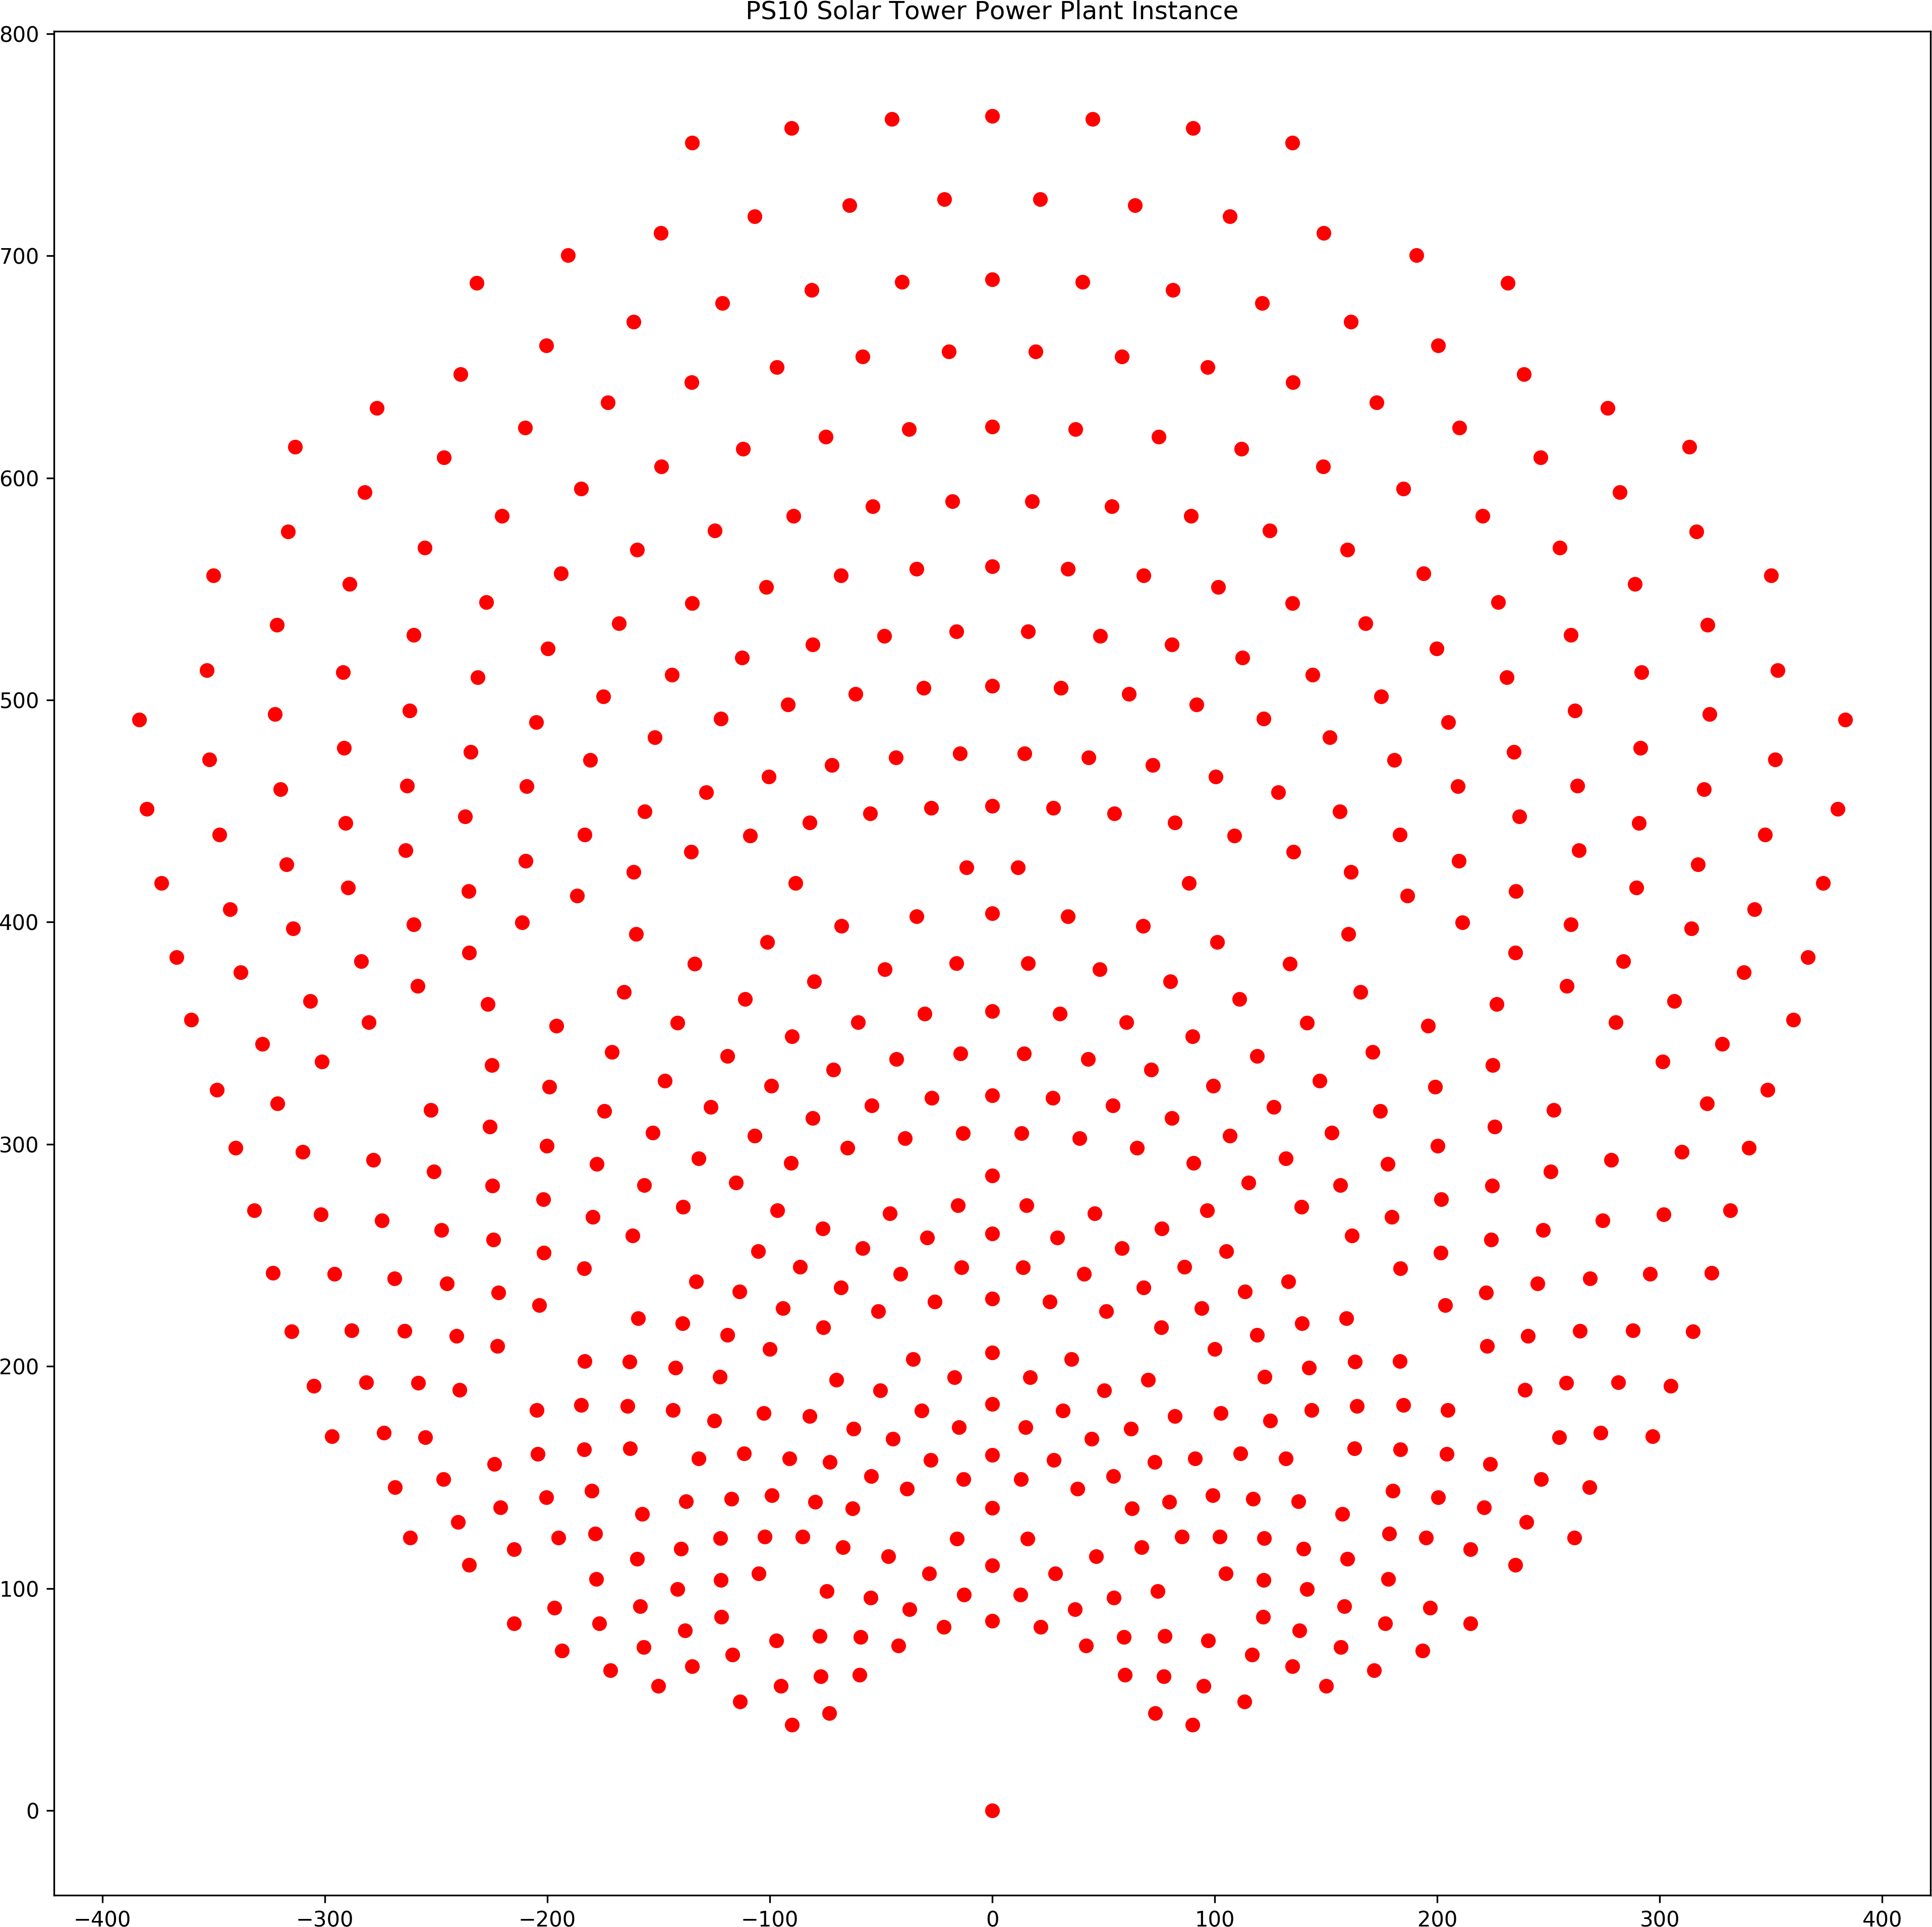
\includegraphics[width=\linewidth]{./img/ps10_instance.png}
  \caption{PS10 instance with its heliostats and the solar tower at coordinate $(0,0)$.}
  \label{fig:ps10}
\end{figure}

\subsection{Trench costs}
For the trench costs we are considering four different costs, each depending on the country we are located in. Each trench has to be constructed by workers and has a depth of 1m as well as 1m in width and length.
  \begin{table}[H]
    \caption{Trench costs for different countries}
    \label{tab:data:trench}
    \begin{center}
    \begin{tabular}{l|c}
      Country & Costs [\euro/m] \\
      \midrule
      Australia & 50 \\
      Spain & 25 \\
      South Africa & 10 \\
      United Arab Emirates & 10
    \end{tabular}
    \end{center}
  \end{table}

\subsection{Data Cable}
  Regarding the data cable we are able to install either a copper or fiberglass cable. The copper cable is much cheaper however it has harsh restrictions regarding its usage, making it only usable for endpoint connections. The fiberglass on the other hand can connect an arbitrary amount of heliostats and has no length restrictions.
  \begin{table}[H]
  \caption{Possible data cables with their cost and restrictions.}
  \label{tab:data:cable}
  \begin{center}
    \begin{tabular}{l|cc|c}
      Data cable type & Max. capacity &  Max. length [m] & Price [\euro/m] \\
      \midrule
      Copper & 2 & 100 & 0.7\\
      Fiberglass & $\infty$ & $\infty$ & 2
    \end{tabular}
  \end{center}
\end{table}

\subsubsection{Local Control Units}
  Exactly one local control units is installed at every heliostat so that communication is enabled. All LCUs with the exception of an endpoint has exactly one ingoing fiberglass cable. The endpoint has exactly one ingoing copper cable.
  \begin{table}[H]
  \caption{Local control units with their degree and cable restrictions for both cable types.}
  \label{tab:data:lcu}
  \begin{center}
    \begin{tabular}{lc|cc|cc}
      LCU type $s$ & Price [\euro/piece] & \multicolumn{2}{c|}{Copper} & \multicolumn{2}{c}{Fiberglass} \\
      && $l_{s,\text{COPPER}}$ & $u_{s,\text{COPPER}}$ & $l_{s,\text{FIBER}}$ & $u_{s,\text{FIBER}}$\\
      \midrule
      Endpoint & 10 & 1 & 1 & 0 & 0 \\
      Conductor & 100 & 0 & 0 & 1 & 2 \\
      8-port copper & 800 & 0 & 7 & 1 & 2 \\
      8-port fiberglass & 800 & 0 & 0 & 1 & 9 \\
      16-port copper & 1500 & 0 & 15 & 1 & 2 \\
      16-port fiberglass & 1500 & 0 & 0 & 1 & 17 \\
    \end{tabular}
  \end{center}
  \end{table}
  Therefore, an 8-port copper LCU for example has up to 7 'outgoing' copper connections and up to one 'outgoing' fiberglass one.

\subsection{Power Cable}
The power cables are not restricted with LCUs. However, maximum capacity constraints have to be taken into account --- as opposed to glasfiber cables that do not have any capacity restrictions. Hence, we have to use more than one power cable for instances with more than 250 heliostats. Therefore we have to partition the heliostats field into partitions that is non-trivial. A simple heuristic is presented in \cref{sec:partitioning}.
\begin{table}[H]
  \begin{center}
  \caption{Power cables with their connectivity limitations and prices.}
  \begin{tabular}{l|cc|c}
    Power cable type & Max. capacity & Max. length [m] & Price [\euro/m] \\
    \toprule
    NYY-J 3x2.5 RE & 56 & 38.36 & 0.58 \\
    NYY-J 3x4 RE & 73 & 47.08 & 0.87 \\
    NYY-J 3x6 RE & 92 & 56.04 & 1.24 \\
    NYY-J 3x10 RE & 124 & 69.30 & 1.95 \\
    NYY-J 3x16 RE & 162 & 84.87 & 3.13 \\
    \midrule
    NYY-J 3x25 RM & 209 & 102.79 & 5.19 \\
    NYY-J 3x35 RM & 250 & 120.31 & 6.90
  \end{tabular}
  \end{center}
\end{table}